\ifdefined\withimages
	\newpage
	\tikz[remember picture,overlay] \node[opacity=1,inner sep=0pt] at (current page.center){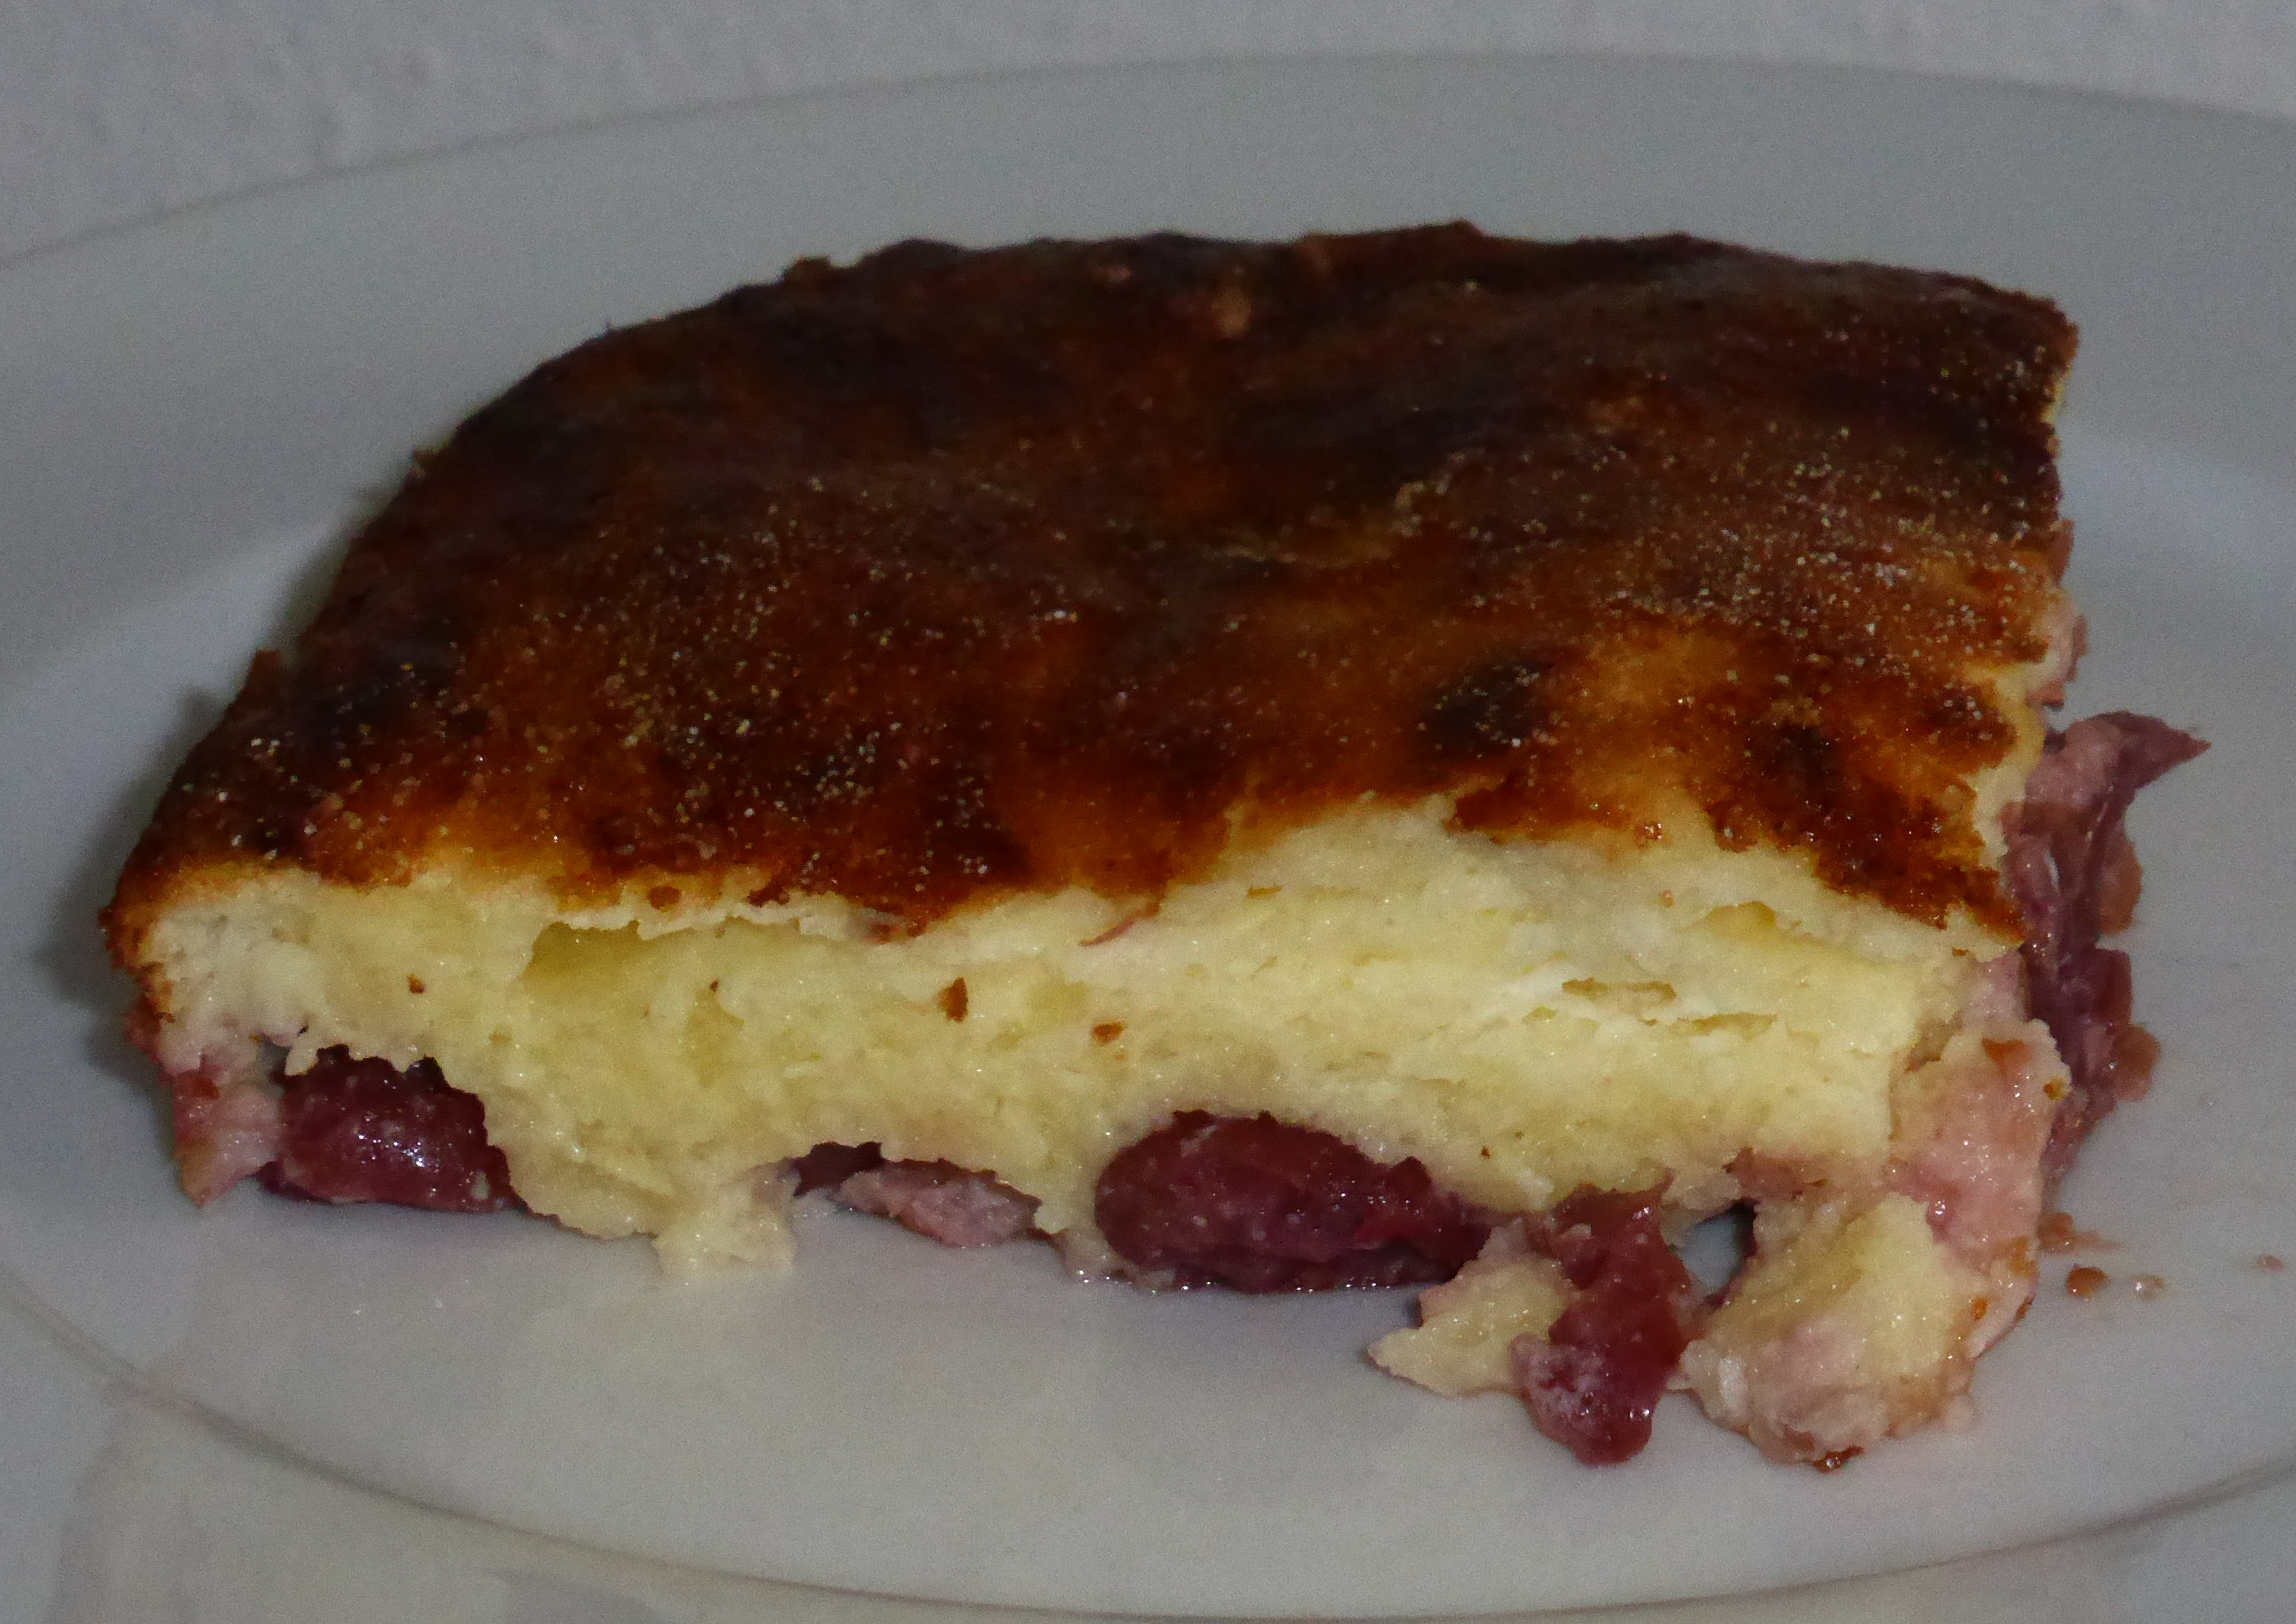
\includegraphics[width=\paperwidth,height=\paperheight]{./bilder/quarkauflauf_ratio.jpg}};
\fi

\begin{recipe}[]{Quarkauflauf} %MUTTI 1
	\timerecipe[Minuten]{ca. 20 + 40} %mit [EINHEIT]
	\personcount[Auflaufform]{1} % mit[ART]
	\ingredient{3 Eier} % ggf. \nicefrac{1}{2}
	\ingredient{75g Butter}
	\ingredient{150g Zucker}
	\ingredient{500g Magerquark}
	\ingredient{40g Speisestärke}
	\ingredient{60g Gries}
	\ingredient{\nicefrac{1}{2}  Päckchen Backpulver}
	\ingredient{1 Glas Kirschen}

\step
Ofen auf 180°C Ober-Unterhitze vorheizen.

\step
\textbf{3 Eier} trennen und Eiweiß steif schlagen.

\step
Eigelb, \textbf{150g Zucker} und \textbf{75g Butter} schaumig schlagen.

\step
\textbf{500g Quark}, die \textbf{40g Speisestärke} und die \textbf{60g Gries} sowie das \textbf{halbe Päckchen Backpulver} untermischen.

\step
Den Eischnee unterheben und auf das \textbf{Glas Kirschen} in die gefettete Auflaufform geben.

\step
Mit \textbf{Butter}flöckchen und \textbf{Semmelbröseln} bestreuen.

\step
Bei 180°C ca. 40 min bei Ober-Unterhitze backen.

%\tippbox{{Tipp:} ...} % Tipp in extra Rahmen
\end{recipe}